% \documentclass[12p]{article}
\documentclass{article}
% bibliographystyle{seg asdf}
% \tiny\bibligoraphy{seq_eg} .bib file
% \usepackage[margin=1in, headheight=110pt]{geometry}
\usepackage[letterpaper, margin=1in]{geometry}
\usepackage{amssymb, amsmath, amsfonts, amsthm}
\usepackage{mathpazo}
\usepackage{setspace}
% \usepackage{probsoln}
\usepackage{fancyhdr}
\usepackage{hyperref}
\usepackage{float}
\usepackage{tikz}
\usepackage{enumitem}
\usepackage{listings}
% \usepackage{lipsum}
\usepackage{parskip} % Use for extra line spacing

\setlength{\parindent}{0 in}

% TODO change these when we figure them out
\newcommand{\namenobold}{Hover Wars}
\newcommand{\name}{\textbf{\namenobold}}
% Darkwire
% Flatlined
% Hot Steel
% Hover Wars    <--- James' pick
% Netrunners    <--- Evan's pick
% Pulse
% Sector 6
% Silver Helix
% Street Warriors
\newcommand{\team}{Team A --- Light Theme is for Heretics}
\newcommand{\botcount}{4}

\pagestyle{fancy}
\lhead{High-level Design}
\rhead{CPSC 585 --- Winter 2019}

\lfoot{\namenobold{}}
\rfoot{\team{}}

\newenvironment{hangingpar}[1]
  {\begin{list}
          {}
          {\setlength{\itemindent}{-#1}%%'
           \setlength{\leftmargin}{#1}%%'
           \setlength{\itemsep}{0pt}%%'
           \setlength{\parsep}{\parskip}%%'
           \setlength{\topsep}{\parskip}%%'
           }
    \setlength{\parindent}{-#1}%%
    \item[]
  }
  {\end{list}}


\newcommand{\sep}{\;}
\newtheorem{theorem}{Theorem}
\theoremstyle{definition}
\newtheorem{definition}[theorem]{Definition}

\newcommand\floor[1]{\lfloor#1\rfloor}
\newcommand\ceil[1]{\lceil#1\rceil}
\begin{document}
\begin{titlepage}
  \begin{center}
    \vspace*{1cm}
    \Large{\textbf{University of Calgary}}\\
    \Large{\textbf{CPSC 585 --- Winter 2019 --- Games Programming}}\\
    \vfill
    \line(1,0){400}\\[1mm]
    \huge{\textbf{\namenobold{}}}\\
    \large{\textbf{High-Concept Design Document}}\\
    \line(1,0){400}\\
    \vfill
    \Large{\textbf{\team{}}}\\
    \Large{Austin Easton, Evan Quan, James Cot\'{e}, Jianan Ding}\\
    \large{January 21, 2019}
    % \today \\
  \end{center}
\end{titlepage}
% \thispagestyle{fancy}
\setcounter{page}{0}
\tableofcontents
\pagenumbering{gobble}
\break{}
\pagenumbering{arabic}
% \onehalfspacing

\section{Introduction}

\begin{figure}[htpb]
  \centering
  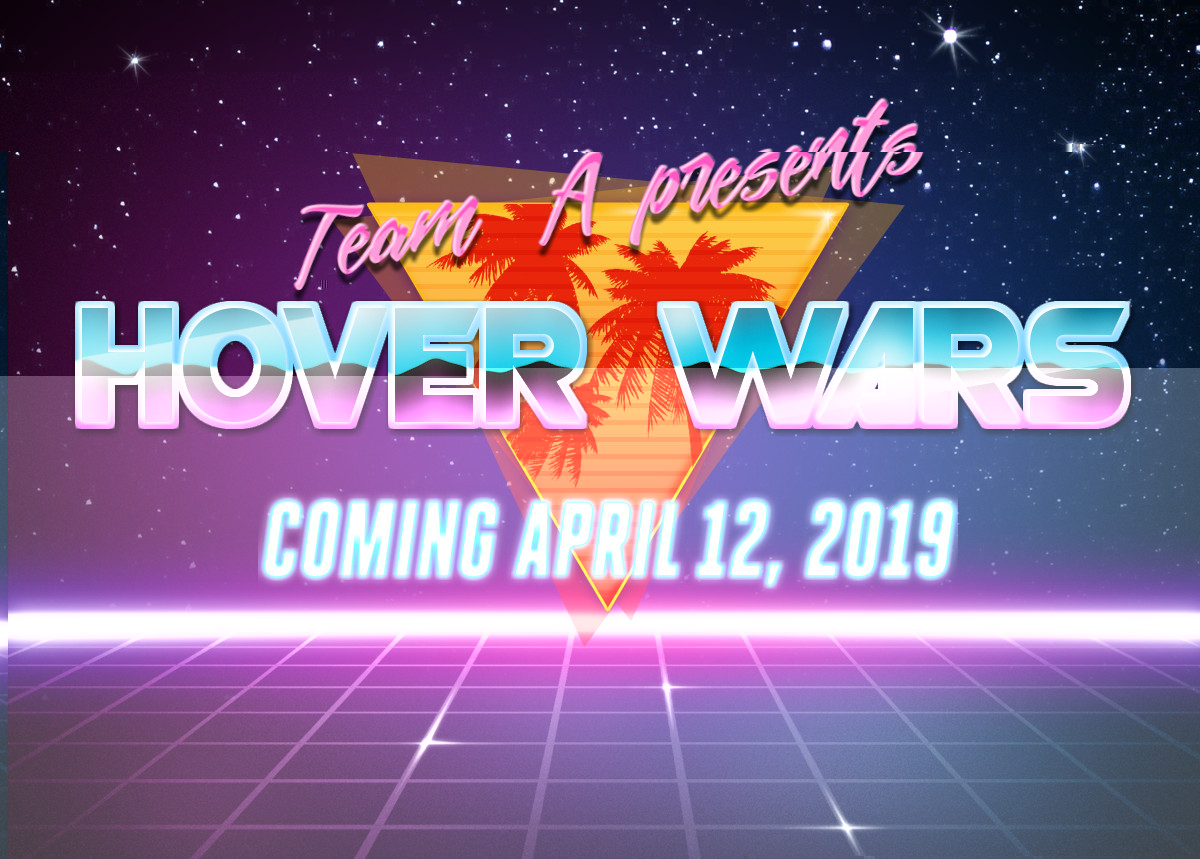
\includegraphics[width=1.0\linewidth]{images/title_art_hover_wars.jpg}
  % 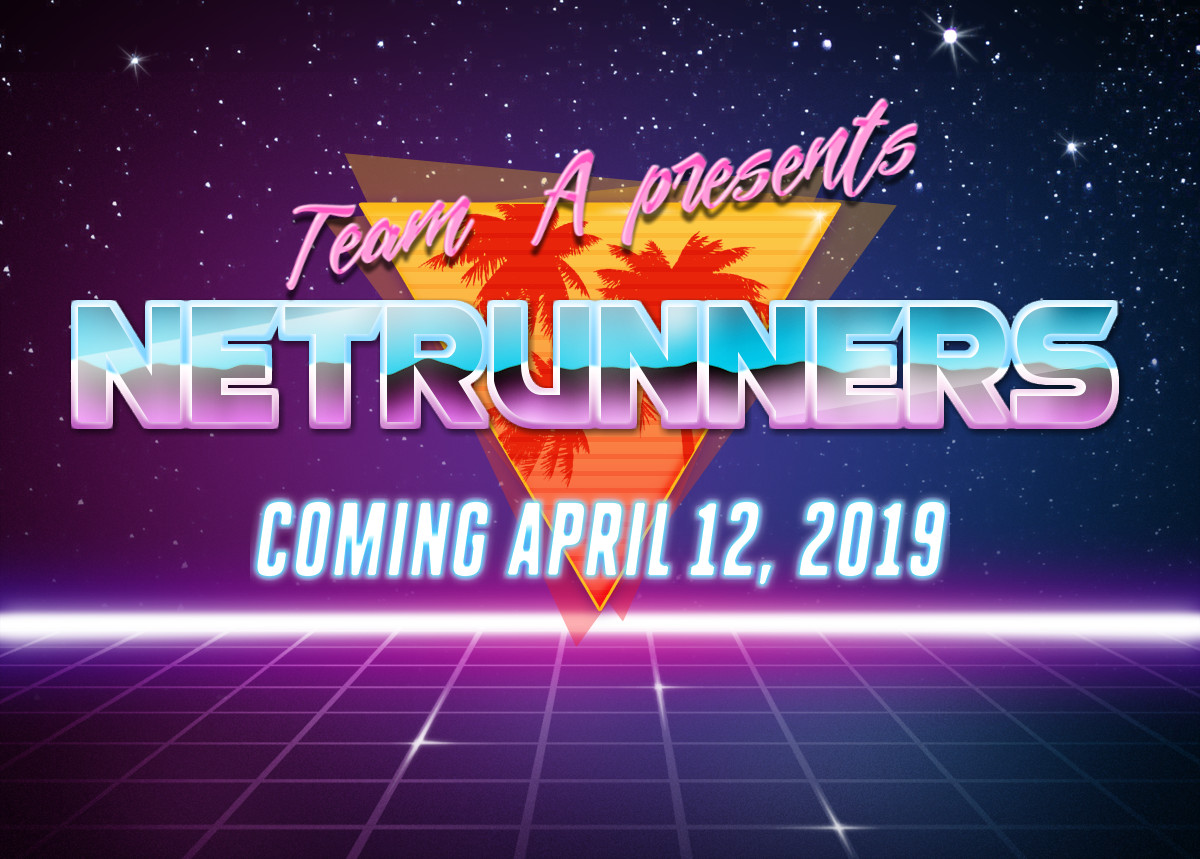
\includegraphics[width=1.0\linewidth]{title_art_netrunners.jpg}
  % \caption{Title_art}
\label{fig:title_art}
\end{figure}

% \begin{figure}[htpb]
%   \centering
%   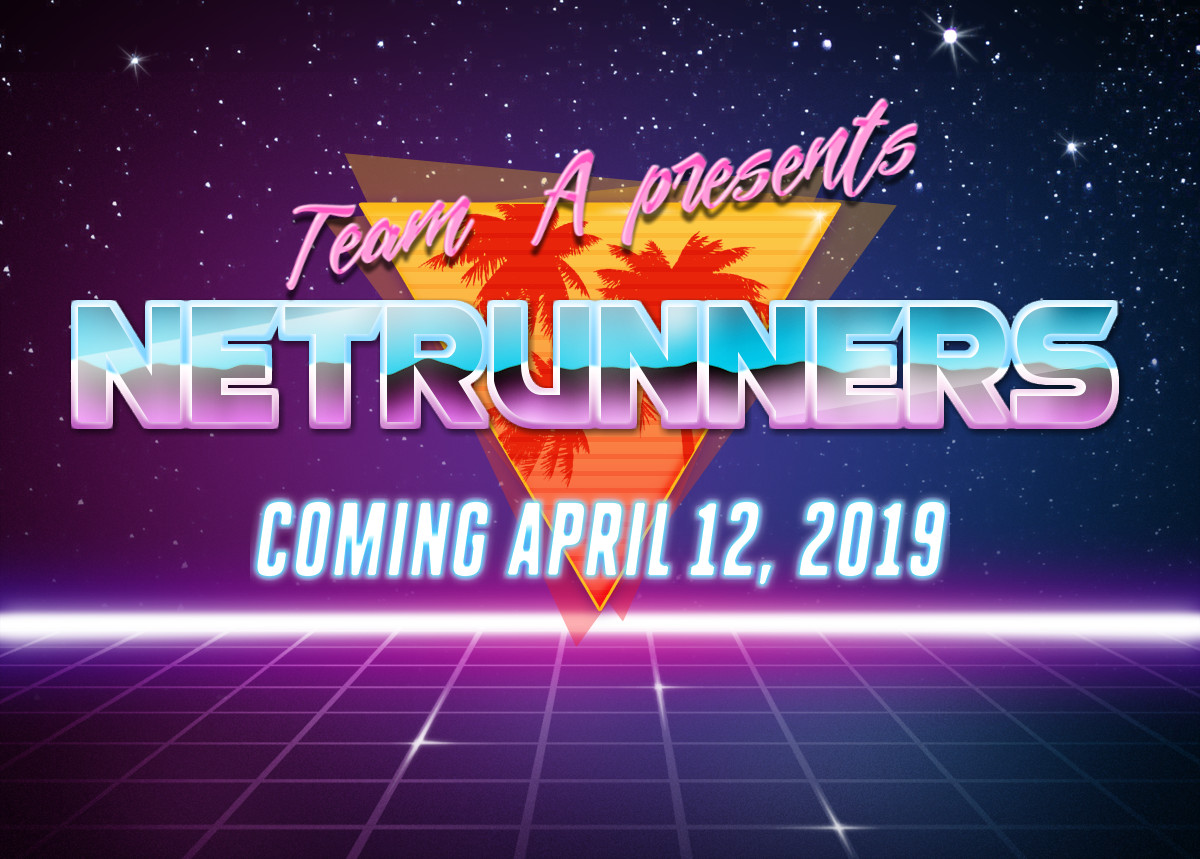
\includegraphics[width=1.0\linewidth]{title_art_netrunners.jpg}
%   % \caption{Title_art}
% \label{fig:title_art2}
% \end{figure}

% TODO king of the hill / secure the intel description
% Netrunners are fighting over valuable intelligence down at sector 6 and are
% causing a scene. Police are on their way to recover it, but are no match
% against your arsenal of weapons. It is up to you to secure the intel against
% your foes to prevent it from falling into the wrong hands.
Autumn 2142. It's the dead of night in the streets of The Grid. You're
blocked off in sector 6 holding stolen intelligence from your latest netrun,
and await as the cops close in from every angle. Alone with your trusty
hovercraft, you must fend off the attack for your dearest life.

\name{} is a combat-based driving game aimed to test your skill and outplay
your enemies. Whether you're playing alone against the AI or against your
friends, each player find themselves driving a hovercraft in an arena pitted
against each other. Utilizing abilities, picking up power-ups, and the
navigating the map, everyone must destroy each other in a chaotic battle of
strategy and wits before the round is over.

The following document details a high-level description of the main gameplay
and game design elements we propose. With the central constraint of these
proposed features being development time available to implement them, the
following features are subject to change as development progresses.

\section{Gameplay}

\subsection{Player Count}

The game supports single and local multiplayer, allowing for 1 to 4 players.
Local multiplayer would be split-screen multiplayer and would require multiple
input devices (XBOX controllers).

\subsection{Game Modes}

The central game mode we propose to implement is \textbf{free-for-all}. At a lower
priority, other modes may be developed if enough time is available.

\subsubsection{Free-for-all}

Each game is composed of a single round that lasts for the duration of a timer.
Each player is placed in an arena to control a hovercraft with various
abilities. They must fight each other in a free-for-all battle with those
abilities, amidst a number of AI-controlled hovercrafts roaming the arena to
hunt down players.

The central goal of the game is to gain the highest score possible before the
round is over. Players have the following means to gain score:
\begin{itemize}
  \item Attacking other player hovercrafts, which can only be done in
    multiplayer. This can be through the use of abilities accessible to every
    player.
  \item Attacking AI-controller hovercrafts (bots), which can be done in both
    single and multiplayer. Bot hovercrafts do not have all the abilities of
    player hovercrafts and so reward less points.
  \item Picking up power-ups. These help the player gain points by improving
    their abilities, but also innately give points when they are picked up.
\end{itemize}

\subsubsection{Secure the Intel Variant 1}

Similar to free-for-all, except a single player is designated to have the
``intel''. Only this player is able to score points, meaning that players must
compete to hold the intel for as long as possible to gain score. If another
player destroys the player holding the intel, that player then takes the intel
and the game continues.

\subsubsection{Secure the Intel Variant 2}

A variation of Secure the Intel merged with free-for-all. All players can gain
points as normal, but the player with the intel passively gains points over
time. This still incentivizes players to get the intel, but still rewards
combat between all the players.

\subsubsection{Secure the Intel Variant 3}

Closer to a classical king of hill style game mode, the first player who holds
the intel for a set amount of time (ex. 2--3 minutes) wins. There is no score
involved as per the other modes, meaning abilities only exist to gain control
of the intel or disrupt other players.

\subsubsection{Free-for-all Survival}

Players only have one life before they are knocked out of the game. The last
player to survive wins the game.

\subsubsection{Co-op Survival}

Players must team up against a never-ending swarm of bots. Players only have
one life before they are out of the game. When all the players are destroyed,
the game ends.

\subsection{Arenas/Maps}

The game will feature a single map. Given the development time frame, a single
fun and polished map is preferable to multiple mediocre maps. It should be
``small'' to ``medium'' in size, to maintain a high player density to ensure
that players are always in the middle of the action and don't feel lost.

\begin{figure}[htpb]
  \centering
  \includegraphics[width=0.8\linewidth]{images/austin_map2.png}
  \caption{A sketch of the map with a more arena-style design.}
\label{fig:austin_map1}
\end{figure}

If time allows for additional maps, they may be added at a lower priority, but
the focus will still be on a singular main map. These additional maps should
provide a different purpose than the main map. For example, there could be
a small map designed for 1--2 players. This will lower the downtime as the
action with be closer and more compact.

\textbf{Primary Environmental Features}

These are basic features that are core to the map's design, and so play a high
priority  in their implementation.

\begin{itemize}
  \item \textbf{Barriers/obstacles} --- These can block movement and
    projectiles. These can take the form of various things: street lamps,
    walls, buildings, tunnels, or other structures.
  \item \textbf{Ramps} --- Ramps lead to higher and lower platforms, or can be jumped
    off of over obstacles. This can provide better vision of certain parts of
    the map, give opportunities to jump between arenas.
\end{itemize}

\textbf{Tentative Environmental Features}

These features are open to be cut, either due to time constraints to implement
or potential game design problems they introduce.

\begin{itemize}
  \item \textbf{Speed pads} --- Driving over these will give a momentary boost of
    speed. Designed for getting power-ups quicker, and chasing or escaping
    other players.

    \textbf{Potential problem:} While these make sense for a racing game, they
    may detract from the gameplay for a combat arena game. Players will
    typically want full control over their vehicle and driving over a speed
    bump in locations where they don't want it can be annoying. If a temporary
    speed boost mechanic is to be implemented, it may be better to have a speed
    boost power-up instead of speed pads.
  \item \textbf{Pits} --- Falling into the pit will instantly destroy the player
    hovercraft. Avoid at all costs or try to bump enemies into it.

    \textbf{Potential problem:} Depending on the placement, size and frequency
    of the pit, players can be easily frustrated if they are constantly
    falling in it. Instant death mechanics such as this can also break the flow
    of gameplay.
  \item \textbf{Jump pads} --- Driving over these, will give a vertical boost
    while maintaining horizontal momentum. Designed for jumping over obstacles
    or reaching areas of higher elevation.

    \textbf{Potential problem:} Similar to speed pads, players may not
    actually want to use them when traversing across the map. It can
    potentially be very disorienting to players to use jump pads, especially if
    they lose control of their movement while in the air. Ramps can serve the
    same purpose without making the player lose control. Anohter possible
    solution would be to allow players to influence their trajectory while they
    are in the air.
\end{itemize}

It is important to note that more features doesn't always mean a better map.
Even if the idea of certain map features are cool or interesting on paper, if
they detract from the overall gameplay experience in practice, it is better to
leave them out. There is value in a good but simple map design.

\subsection{Hit Points, Lives, and Damage}

There are a few hit point and damage systems we have considered. We are
currently committed to implement the \textbf{hit and continue} system, but will
be open to change as we play-test.

\subsubsection{Hit and Continue}

Modelled after \textbf{Mario Kart}'s damage system, hovercrafts are blown away or
spun around when they are hit by abilities, temporarily making the player or
bot that was hit lose control of their vehicle. Shortly afterwards, control is
regained and the hovercraft is given a few seconds of invincibility before
continuing on playing. This minimizes the downtime during play since there is
no respawning, while still punishing players that get hit. It also avoids the
disorienting effect that respawning can have, especially if the map is not
familiar to the player.

\subsubsection{Lives with Hit Points}

Players start the game alive with a small set amount of hit points, which will
be explicitly displayed to the player. They can be damaged by the abilities of
other hovercrafts, lowering their current hit points. The same temporary loss
of control will occur as the hit and continue system. When all hit points are
removed, the player's hovercraft is destroyed.

When a player's hovercraft is destroyed, they are momentarily out of the game
before respawning randomly at one of the respawn points on the map. If another
player destroyed said hovercraft, that player is awarded points for the kill.

Under this system, bots could have fewer hit points than players.

\subsubsection{One Hit One Kill}

Similar to the lives and hit points system, but players are instantly destroyed
upon impact of an ability. This makes getting hit more punishing and further
promotes players to dodge abilities.

\subsection{Players}

\begin{figure}[htpb]
  \centering
  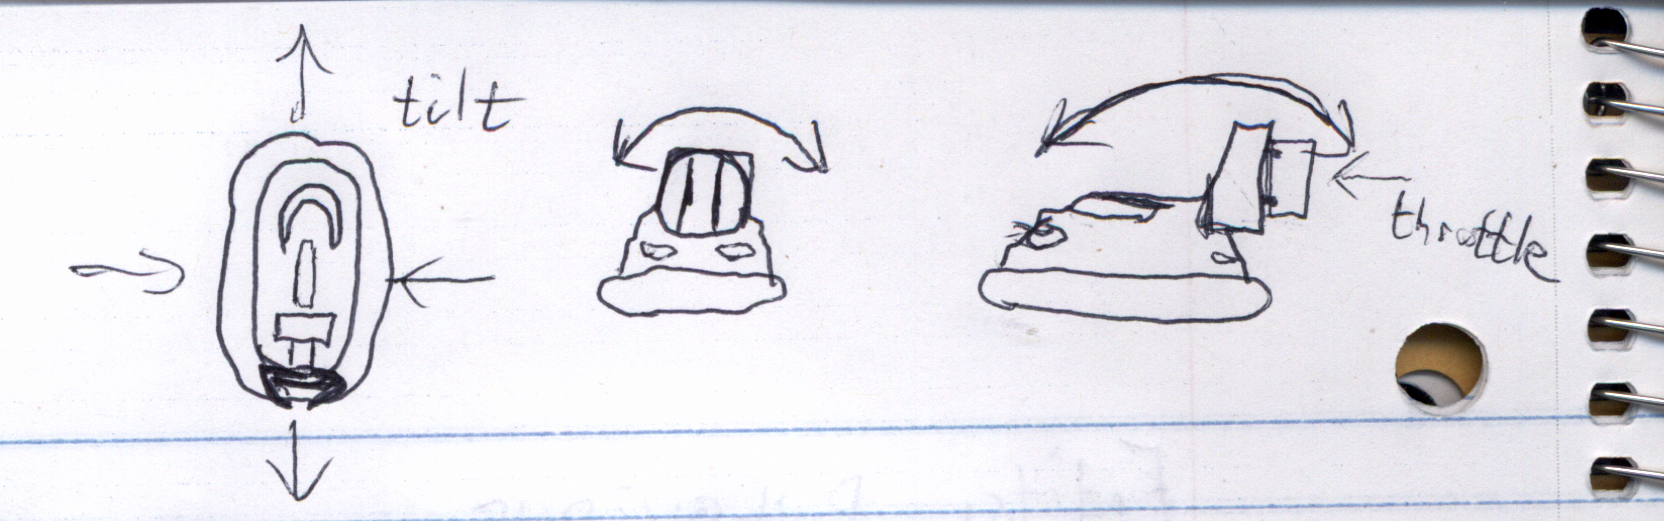
\includegraphics[width=0.8\linewidth]{images/Brainstorming_003.png}
  \caption{Sketch of the player hovercraft with a more mechanical, used-future
  design.}
\label{fig:Brainstorming_003}
\end{figure}

\begin{figure}[htpb]
  \centering
  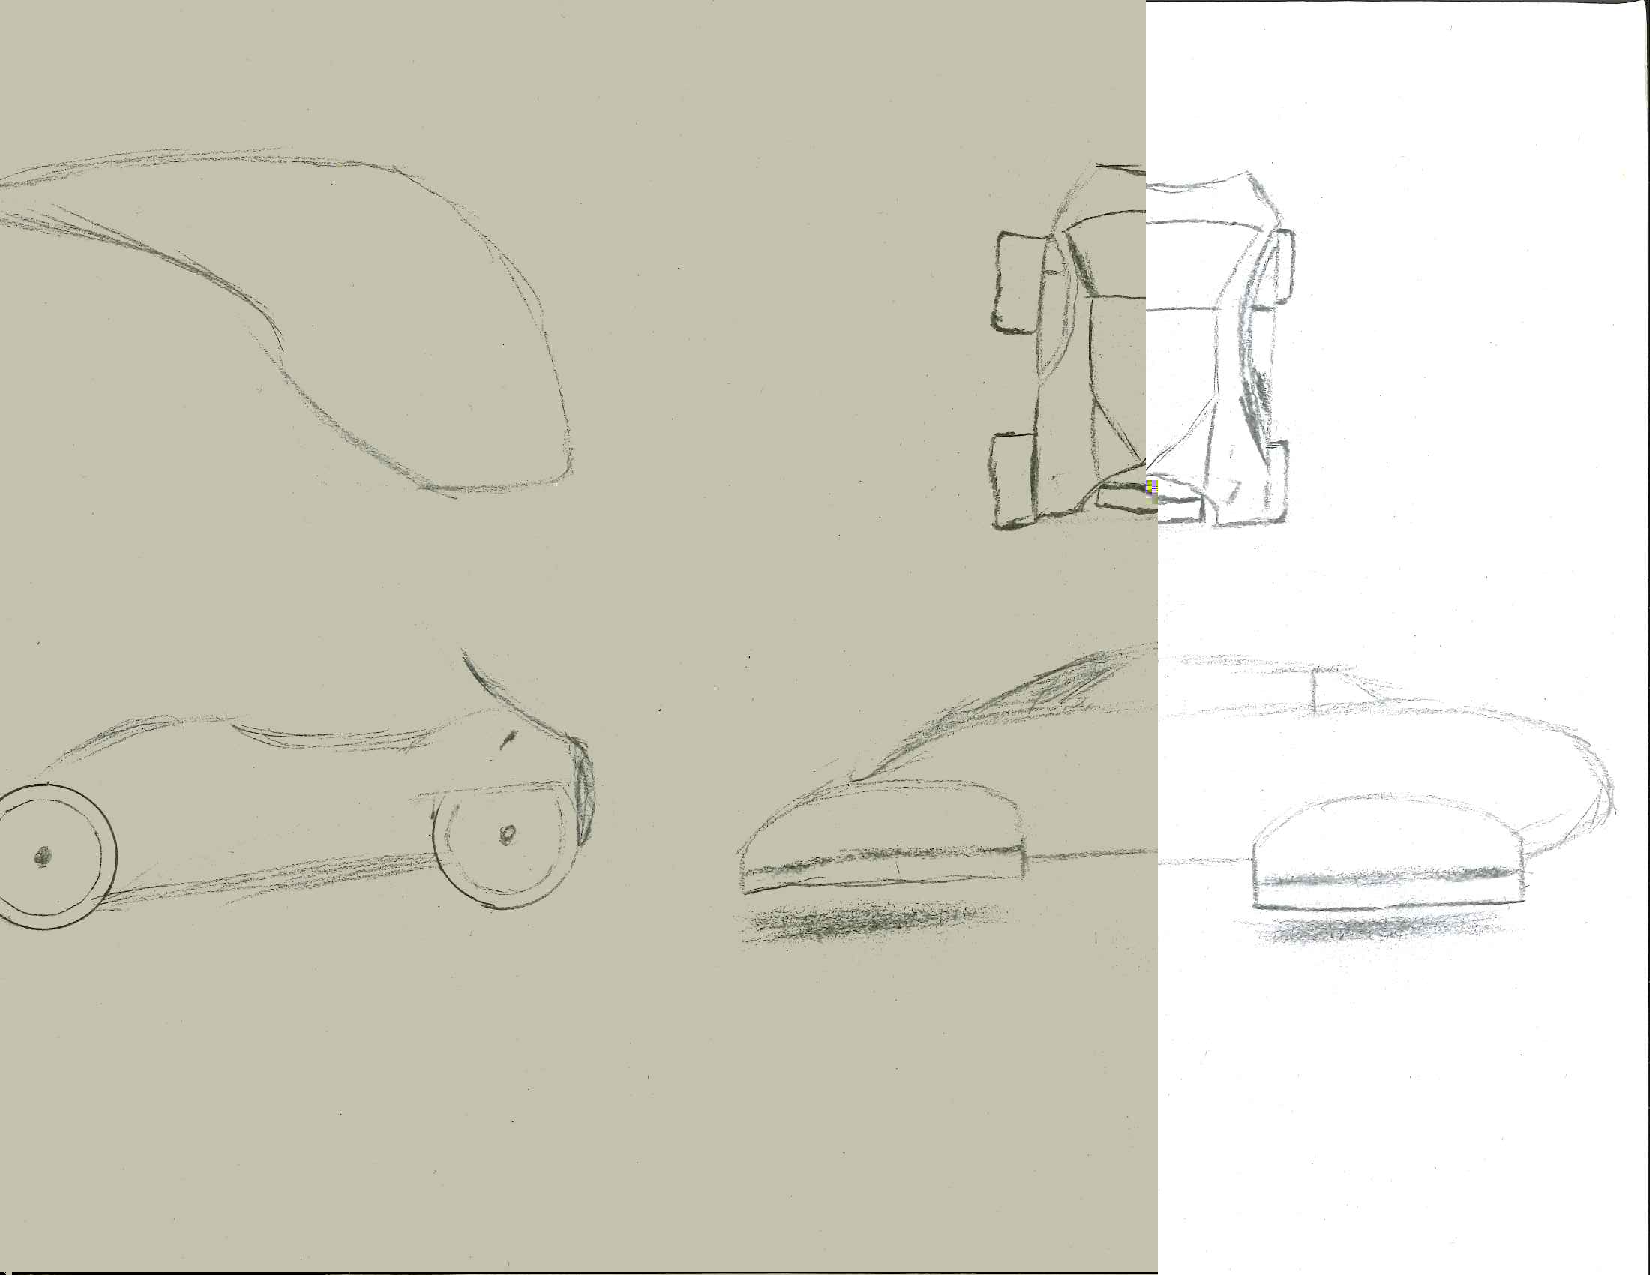
\includegraphics[width=0.8\linewidth]{images/austin_car1.pdf}
  \caption{Sketch of the player hovercraft with a sport car-like design.}
\label{fig:austin_car1}
\end{figure}

Players drive a hovercraft. They innately have full access to a number of
movement options and abilities from the start of the game.

\subsubsection{Movement}

\begin{itemize}
  \item \textbf{Standard movement} --- A hovercraft does not rely on wheels to
    move and so can traverse in any lateral direction without needing to turn,
    meaning that strafing is possible.
  \item \textbf{Acceleration/braking} --- A hovercraft can accelerate an brake
    in any direction is it currently moving. It will often drift if a turn is
    made, even at relatively slow speeds, which can be both advantageous and
    disadvantageous. This is open to change as movement is play-tested to
    figure out what is fun and feels right.
  \item \textbf{Dashing} --- A hovercraft can dash in any direction. From
    a mobility standpoint, dashing can be used to catch up to other
    hovercrafts, reach power-ups faster, or lose others when being chased. From
    a defensive standpoint, it can be used to dodge attacks.
\end{itemize}

\subsubsection{Abilities}

Every hovercraft has 3 attack abilities that are available from the start of
the game.

\begin{itemize}
  \item \textbf{Rocket} --- A rocket launches forward straight out from the
    direction the hovercraft is facing until it hits a surface. Upon impact, it
    explodes, damaging everything in a radius around it. Being the only ranged
    attack, it is great for attacking distant enemies if aimed well, or when
    chasing other vehicles. The splash damage can be utilized with parts of the
    arena environment to hit enemies near walls easier, or to hit multiple
    enemies that are grouped together.
  \item \textbf{Spikes} --- Spikes temporarily extend in all directions from
    the hovercraft, damaging other vehicles that come in contact with it. Can
    be used both aggressively and defensively when other vehicles are nearby.
    It can also be used in combination with dashing to crash into enemies.
  \item \textbf{Trail} --- A trail is created on the ground behind the player.
    Any hovercraft that contacts it is damaged. After some time, the trail
    eventually disappears. Great to use when being chased. Visually, this trail
    may be composed of flaming napalm, light energy, or some toxic substance,
    which is still up for discussion as development continues. Players can dash
    through the trail unharmed.
\end{itemize}

\subsection{Bots}

In all modes, a number of AI-controlled hovercrafts, or bots, will be present
on the map. With a visually distinct design from players, bots will only target
player hovercrafts. They are weaker than players in that they have fewer hit
points and fewer abilities, but also award less points on kill. As a result, it
is up to players to decide much they want to focus on destroying bots versus
other players in their strategy.

The number of bots present in the game as well as their capabilities is
open-ended as development progresses. Here is a tentative priority list of bot
functionality, from highest to lowest priority.

\subsubsection{Movement}

It will be a requirement for bots to be able to target players to chase them.
They must be smart enough to recognize the presence of obstacles and general
map geometry to reach players in a reasonably direct path if possible.

At a lower priority, they may be given movement abilities or have more advance
movement decision-making such as:
\begin{enumerate}
  \item Speed boost. Bots will accelerate towards players when a clear path is
    between the two of them. This will help them use their spikes to crash into
    the player for damage.
  \item Guard power-ups. Bots will recognize when power-ups are on the map and
    prioritize attacking players who they believe are going for them.
\end{enumerate}

\subsubsection{Abilities}

To work with their basic chasing behaviour, the bots will, at minimum, be
equipped with the spikes ability, allowing them to ram into the player for
damage. Whether the spikes need to be activated or are always enabled will be
up to play-testing.

At a lower priority, they may given other abilities like the players:
\begin{enumerate}
  \item \textbf{Rockets} --- At its simplest, bots would be able to aim at
    players to fire rockets at them. More sophisticated, bots would be able to
    lead their shots based on the player's predicted trajectory and the rocket
    trajectory. They may also utilize walls to hit players with the rocket's
    explosion radius. Bot rockets may potentially travel slower than player
    rockets.
  \item \textbf{Dashing} --- Bots would be able to dash out of the way to dodge
    abilities.
  % \item \textbf{Trail} --- Bots will try to intercept the player's path to get
  %   them caught in the trail. This is
    % TODO remove this, too difficult
\end{enumerate}

\subsubsection{Friendly fire}

Since the bots team up against the players, any damage they would deal to each
other would be purely accidental. At first glance, it would seem reasonable to
disable friendly fire so that bots would not destroy each other en masse.
However, friendly fire amongst bots may create in-game situations that would
add extra chaos, excitement or even humour to the game's atmosphere. If need
be, the bot count (or respawn timing if hovercraft destruction is implemented)
would be adjusted for balance to account for these friendly kills.

Ultimately, the decision for allow for bot friendly fire will be up to
play-testing, and we will be open for it to work either way.

\subsection{Power-Ups}

Throughout the map, there are set power-up spawn locations that will randomly
spawn one of several power-ups. Players can pick them up by contacting them.
Upon contact, the player that picked it up will temporarily receive passive
bonus for a set duration.

At minimum, we want there to be 3 total power-up types. While there is no
particular priority in what power-ups to implement, we would ideally have one
power-up for each player ability. Here are some ideas:

\textbf{Rocket}
\begin{itemize}
  \item \textbf{Rapid-fire rockets} --- Rockets can be launched at a faster rate of
    fire. Good for spamming at a distance.
  \item \textbf{Explosive rockets} --- Rockets will have a much larger impact
    radius. Good for taking out groups of enemies in small corridors.
  \item \textbf{Multi-rockets} --- Shoot multiple rockets at once.
\end{itemize}

\textbf{Spikes}
\begin{itemize}
  \item \textbf{Large spikes} --- Spike size increases, hitting enemies are
    further distances.
  \item \textbf{Longer spike duration} --- Spike duration is increased.
  \item \textbf{Bumper spikes} --- When enabled, the player is immune to other
    players' spikes.
\end{itemize}

\textbf{Trail}
\begin{itemize}
  \item \textbf{Wide trail} --- The trail is much wider, easing the ability to
    catch opponents in their tracks.
  \item \textbf{Longer trail duration} --- The trail continuously lasts on the
    map for the duration of the power-up.
  \item \textbf{Slowing trail} --- The trail slows the movement of enemies
    crossing it, making them vulnerable to attack.
  \item \textbf{Blocking trail} --- The trail cannot be bypassed, blocking
    enemies trying to cross it. Great for defense when being chased, or
    aggressively to trap enemies in an area.
\end{itemize}

\textbf{Other}
\begin{itemize}
  \item \textbf{Repair} --- The player gains an extra hit point. This obviously
    would only exist if we decide to implement a hit point system.
  \item \textbf{Speed boost} --- The player gains a speed boost.
  \item \textbf{}\textbf{Shield} --- The player is invulnerable to abilities.
  \item \textbf{Invisibility} --- The player is invisible to other players and
    will not be targeted by bots.
\end{itemize}

\subsubsection{Spawning}

There are three power-up spawning systems we believe are workable, each with
their pros and cons:

\begin{enumerate}
  \item \textbf{Random Unknown} --- When a power-up spawns, it is unknown to
    the players what power-up type it is until it is picked up.

\begin{figure}[htpb]
  \centering
  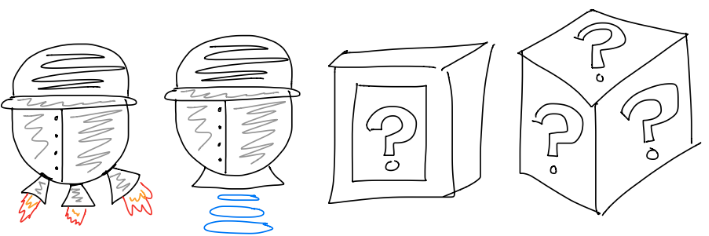
\includegraphics[width=0.8\linewidth]{images/powerups_unknown.png}
  \caption{Concept art of power-up appearance if unknown to player.}
\label{fig:powerups_unknown}
\end{figure}

    \textbf{Pros:} This can add a sense of surprise to the players as they find
    out what power up they have. It can also change up the gameplay as players
    adapt their strategy to best utilize whatever power-up they have gained.
    This prevents players from just taking a single type of power-up.

    \textbf{Cons:} May not be as interesting as the other systems.
  \item \textbf{Random Known} --- When a power-up spawns, it is randomly chosen
    from the list of possible power-ups and is known to the player what
    power-up type it is by its appearance.

    \textbf{Pros:} This can add an extra layer of strategy as players can
    scout the map for power-ups they they want, if certain ones work better
    for their play style or current strategy.

    \textbf{Cons:} If certain power-ups are deemed useless or underpowered,
    then no players may pick them up. Over the duration of the round, all
    power-up locations may eventually be filled up with those power-up types as
    players ignore them.
  \item \textbf{Deterministic by location} --- Certain parts of the map
    deterministically spawn certain power-up types.

    \textbf{Pros:} This can add an extra layer of strategy as players can
    gravitate towards certain areas to get certain power-ups they want.

    \textbf{Cons:} Certain areas of the map may be neglected if they have bad
    power-ups.
\end{enumerate}

\begin{figure}[htpb]
  \centering
  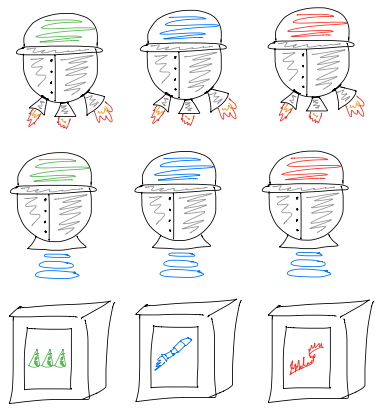
\includegraphics[width=0.8\linewidth]{images/powerups_known.png}
  \caption{Concept art of power-up appearance. Certain colours correspond to each ability.}
\label{fig:powerups_known}
\end{figure}


As it stands, we are committed towards the \textbf{Random Unknown} spawning
system, but will be open to change as we play-test.

\subsection{Difficulty}

\textbf{Single Player}

In a single player experience, the difficulty can arise
from a competitive approach in achieving a high-score. Whether one is
attempting to outperform their previous high scores, or compete with others'
high scores, players can improve their skills and learn new strategies to
improve. This self-imposed motivation to improve and compete can create new
levels of difficulty at a meta game level.

\textbf{Multiplayer}

Similar to single player, difficulty arises from the skills of opposing
players. As other players improve, so does oneself need to do to so to compete.
New strategies can arise in using abilities, power-ups, and parts of the map to
maximize points, as well as strategies to counter other players' play styles.

\subsection{Menu}

\section{Game Design}

\subsection{Aesthetic}

Visually, the game mainly follows a cyberpunk and Tron aesthetic. We are going
for a futuristic city at night appeal.

\begin{figure}[htpb]
  \centering
  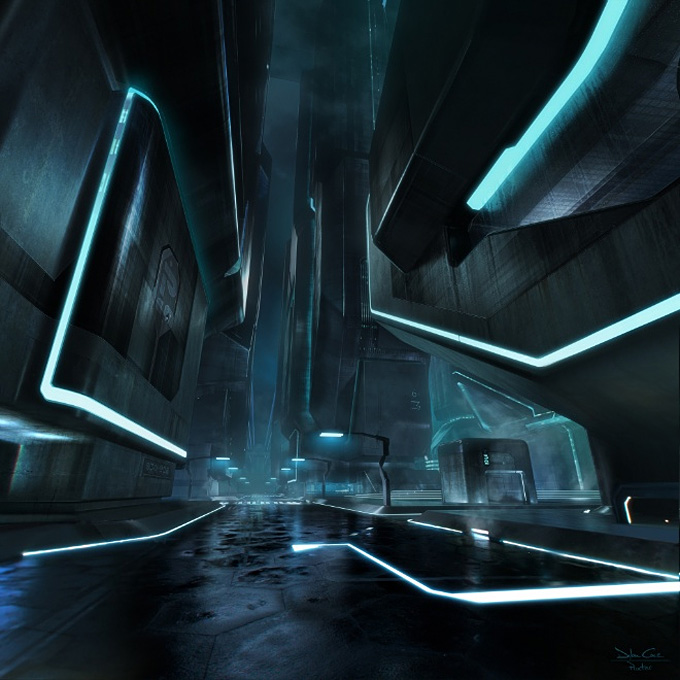
\includegraphics[width=0.8\linewidth]{images/theme01.jpg}
  \caption{Taking place at night, there will be a focus on artificial lights
  from buildings to illuminate the area.}
\label{fig:theme01}
\end{figure}

\begin{figure}[htpb]
  \centering
  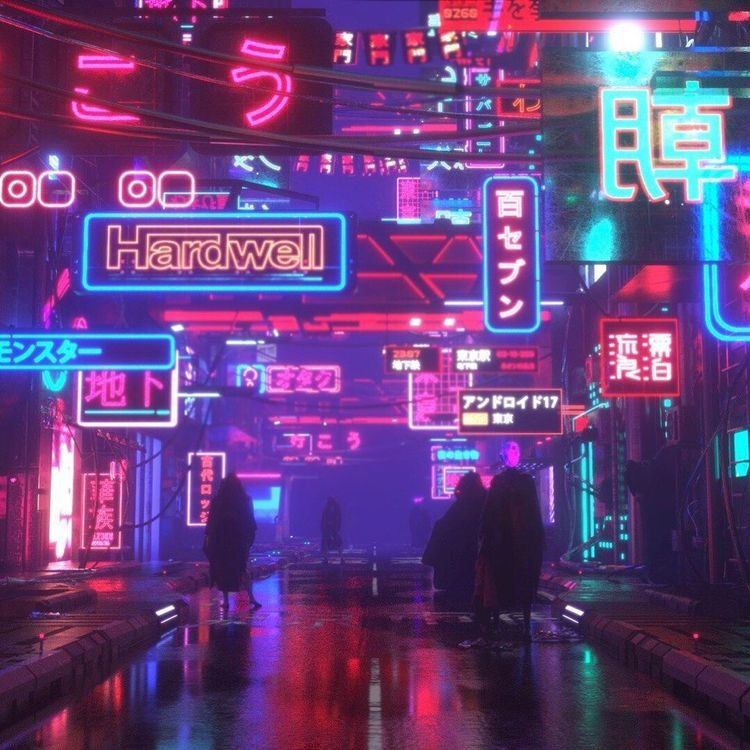
\includegraphics[width=0.8\linewidth]{images/theme02.jpg}
  \caption{Colourful neon lights will play an important role in creating
  a sense of warmth.}
\label{fig:theme02}
\end{figure}

\begin{figure}[htpb]
  \centering
  \includegraphics[width=0.8\linewidth]{images/theme03.jpg}
  \caption{There may be a contrast of lighter and darker arenas in the map,
  which may be used to highlight important areas such as power-up locations, or
ramps leading to different areas.}
\label{fig:theme03}
\end{figure}

\subsection{Inspiration}

\name{} is inspired from a number of other games:
\begin{itemize}
  \item \textbf{Akane} (2018) --- aesthetic
  \item \textbf{Counter-strike} (2000) --- point system
  \item \textbf{Crawl} (2017) --- secure the intel game mode
  \item \textbf{Cyberpunk 2020} (1990) --- aesthetic
  \item \textbf{DOTA 2} (2010) --- point system
  \item \textbf{Mario Kart} (1992) --- free-for-all game mode and general combat design
  \item \textbf{Pac-Man} (1980) --- bot versus player design
  \item \textbf{ThinkTanks} (2003) --- speed and jump pads
  \item \textbf{Tron} (1982) --- aesthetic and trail ability
\end{itemize}

\subsection{Designer Insight/Goals}

Here are some goals we have in mind for the project, as well as some insight
behind our design decisions from our team discussions.

\subsubsection{Vibe}

Playing \name{} should feel exciting and bring a sense of hype and energy,
similar to combat games like \textbf{Super Smash Bros} or \textbf{Street
Fighter}. This can be brought about through fast-paced gameplay, coupled with
action-packed sound effects and music.

\subsubsection{Role of AI}

The introduction of AI-controlled hovercrafts (bots) adds an interesting
element to the game, but also a few problems.

First, given our past experience and the time-frame creating the AI, we don't
believe the bots will be equally competent to a skilled human player. If bots
are given a hovercraft with equal capability to that of a player, it is
unlikely they will be able to utilize their abilities and movement sufficiently
to compete with players, or have sufficient game sense to outplay and counter
different play styles. This poses a problem for single-player, as competing
against a group of underperforming bots will not particularly fun or
challenging.

To address the challenge issue, it is possible to give bots point bonuses when
they score to improve their chances to beat players. However, this does not
necessarily address the fun issue, as the player will still experience fighting
against simple bots.

Instead, bots can be given an alternative role rather than replacing a player.
By explicitly giving them less capabilities than the player, and having them
exist in-game independent from the player count, they can add an extra depth to
the gameplay without heavily relying on the depth of their capabilities. The
benefit is that if the bots end up less capable than we initially planed, the
combat can still be just as fun since bots will be in greater numbers and team
up against the players. If they are more capable than we initially planned then
all the better, since this will simply make the gameplay more engaging.

Overall, the focus of multiplayer will be on the interactions between players
for the multiplayer experience, where the bots will provide a background or
secondary element to the gameplay. For single player, the bots will be core to
the gameplay, as they are the only enemy against the player.

\subsubsection{Driving System}

Since players are driving hovercrafts, the driving experience should model
that of a hovercraft. As a result, the driving model should feel somewhat
floaty, allowing for easier drifting. Without the constraint of wheels, the
players should be able to move in any lateral direction without needing to
turn, allowing for strafing.

However, if the hovercrafts are too floaty, they may be frustrating to control.
Driving needs to feel responsive, especially if sudden turns or braking are
done. Our decision to add the dashing mechanic partially solves this problem,
allowing for players to make sudden movements to combat times when they may
feel out of control.

Our goal is for there to be a balance in the driving system for it to feel
somewhat floaty to imitate a hovercraft, and yet grounded enough to feel fun
and responsive. As we play-test the movement throughout the development, we
will iterate on this balance, and may even radically change how driving feels
if we believe it is best for the game.


\subsubsection{Learning Curve}

\textbf{Easy to Learn}

A core goal for game is for it to be easy to pick up and start playing.
Part of this involves controls that are intuitive to new players. While there
are a fair number of abilities, they are the same for everyone, meaning players
do not need to know the ins-and-outs of different vehicle abilities that they
themselves do not have access to.

Power-ups should feel intuitive to understand and use. They should not
introduce new mechanics or keybindings. It is frustrating for new players to
``waste'' power-ups in order to understand what they do, especially if they are
single-use. Instead, power-ups should augment already existing abilities and
clearly display in the UI which ability is improved.

\textbf{Hard to Master}

Players should be given opportunities to improve and apply their skill. Each
ability is distinct and require their own skills to use. Players can learn
which abilities fit well for what situations and adapt to different playstyles.
Various strategies on map control can be learned to gain power-ups easier or
deny them to enemies. While \name{} is not primarily geared towards highly
competitive play, we think its important to consider how the game could play at
a competitive level when designing and balancing elements of the game.

\subsubsection{Getting Hit}

Independent of which damage system we implement (hit and continue, lives with
hit points, or one hit one kill), we want to ensure that it is in line with
number of our design goals.
\begin{itemize}
  \item \textbf{Emphasize the impact of getting hit} --- Getting hit should
    feel bad. It should be immediately noticable to the player and have
    a sizeable in-game impact more than just altering points on the scoreboard
    or decrementing hit points. A temporary loss of vehicle control is enough
    to get the player's attention (along with any accompanying visual and audio
    effects), and punishing enough for them to want to avoid getting hit.

    This system would be constrasted with damage systems found in some first or
    third-person shooters, in which players may receive a number of hits with
    either no or minimal in-game effects, allowing them to ``tank'' damage.
  \item \textbf{Ease user memory load} --- Players do not need to concern
    themselves with the stats of various abilities with how much damage they
    each do. By keeping it simple to either getting hit with an abilitiy or
    not, players simply need to know a single general rule of the consequence
    of receiving damage.
  \item \textbf{Easy to Interpret} --- It is easier to understand how much
    damage the player can take if hit points are described in small values (ex.
    3), or if there is no hit point system at all. As the player's immediate
    attention is on the action in front of them, they should perfectly
    understand the state of their hovercraft at a moment's glance, without
    needing to read large numbers or perfect rough calculations.

    For example, with a health bar, a percent gauge, or larger hit points
    values (ex. 100), players may have some rough idea how many hits can can
    take, but it can still be somewhat fuzzy if abilities deal different
    amounts of damage, or if players need to figure out how many more hits they
    can take from how much damage different abilities do.
\end{itemize}

\subsubsection{Abilities}

In designing our abilities, we have several goals in mind. For each one
included, we want to make sure that they:
\begin{itemize}
  \item \textbf{Feel distinct to use:} They should employ different strategies
    to use in order to feel unique. Abilities that are too similar can be
    boring.
  \item \textbf{Serve different purposes:} Multiple abilities that are
    best-used for the same situations creates redundancy. Either both abilities
    are equally useful in those situations, making having both unnecessary, or
    one is better than the other, making the other obselete.
  \item \textbf{Introduce some level of counterplay:} If skilled enough,
    players on the receiving end should be able to avoid getting damaged if
    they react appropriately. Not being able to react to abilities can feel
    cheap and frustrating, especially if they recognize what ability is about
    to be used and feel helpless to respond. As a result, we have avoided all
    hitscan weapons as they cannot be doged and can be difficult to anticipate.
  \item \textbf{Are deliberate in their use:} Due to the health and damage
    system we plan to implement, abilities are viewed more more from a ``hit or
    miss'' view rather than ``receive various levels of damage'' view. So just
    as abilities require attention to identify and avoid from the receiving
    end, they should also require a similar amount of attention to use from the
    aggressor's end. Players should have to identify their targets and employ
    some amount of skill to correctly hit their enemies, whether it involves
    aiming, colliding with or maneuvering around enemies. As a result, we have
    avoided abilities with high rates of fire that are easily spammable, or
    ``fire and forget'' weapons that do not require much thought to use.
\end{itemize}

These goals will always be in mind if we decide to create additional new
abilities or tweak the existing ones later down the road.

\subsubsection{Blue Shell Effect}

In the context of this game, the blue shell effect can be described as
\textit{``a mechanism that evens the playing field between players that are
performing well and those who are not''} in reference to the infamous blue
shell item in \textbf{Mario Kart}. It gives players that are behind a chance to
comeback in order to make games closer. Most multiplayer games implement some
level of blue shell effect in their game mechanics, some through ``better''
means than others. There are a few common rationales for why this is desirable:
\begin{enumerate}
  \item This can make the game more fun for less-skilled players by
    easing their ability to compete with higher-skilled players (hopefully not
    in an over-corrective manner if tweaked properly).
  \item In games where players' abilities or stats can improve over time due to
    player actions/decisions (through items, power-ups, etc.), those who are
    ahead can easily snow-ball out of control, as their current power lead can
    further help them create an even bigger power lead. Blue shell mechanics
    can help combat snowballing.
\end{enumerate}

A blue shell mechanic we want for the game would be to track player
kill-streaks, which is the number of kills (hits) they have done to other
players in a row without getting hit themselves. As the kill-streak increases,
so does a bounty on that player. If another player kills that player with
a bounty, they are awarded extra points. This makes players that are performing
well higher priority targets, while not giving them a direct gameplay
disadvantage that seems unfair. We may experiment with other systems as we
play-test if we feel like it could be improved or better balanced.

\subsubsection{Performance}

\begin{itemize}
  \item \name{} should run at 60 fps for single player and 30 fps for
    4-person multiplayer.
\end{itemize}

\subsection{Market Competition}

The main competition with \name{} in the market is Nintendo's \textbf{Mario Kart}
franchise, which \name{} is heavily inspired from. As a fairly popular
franchise, we hope to differentiate our game by emphasizing the combat aspect,
as \textbf{Mario Kart} is primarily racing game first.

Another game that would compete with \name{} would be \textbf{ThinkTanks},
developed by GarageGames in 2003, which also plays as a vehicle-based battle
arena game. Our edge over \textbf{ThinkTanks} would be the greater ability
diversity and faster-paced gameplay, which will hopefully draw a greater
appeal.

\subsection{Game Genre} % Is this needed?

\name{} is a third-person combat-based driving game. It is designed to be
a fun party game that is easy for new players to pick up and play, while giving
the opportunity to those who want to master it the means to do so given.

It is developed for the PC, supporting Windows as a high priority and Mac and
Linux with lower priorities, using mouse and keyboard controllers. It will also
support XBOX 360 controller support, allowing for multiplayer modes.

\subsection{Branding}

\name{} is a new IP on its own.

\subsection{Target Market}

While violence is a core component of the gameplay, nothing is particularly
graphic due to the use of vehicles and the lack of blood and gore. We do not
intend there to be any mature themes in the game. We therefore believe that
\name{} is appropriately targeted for all ages 10 and above years of age.

\section{Concept Art}

\begin{figure}[htpb]
  \centering
  \includegraphics[width=0.8\linewidth]{images/Brainstorming_001.png}
  \caption{Rough sketches of the map, UI, and hovercraft}
\label{fig:Brainstorming_001}
\end{figure}

\begin{figure}[htpb]
  \centering
  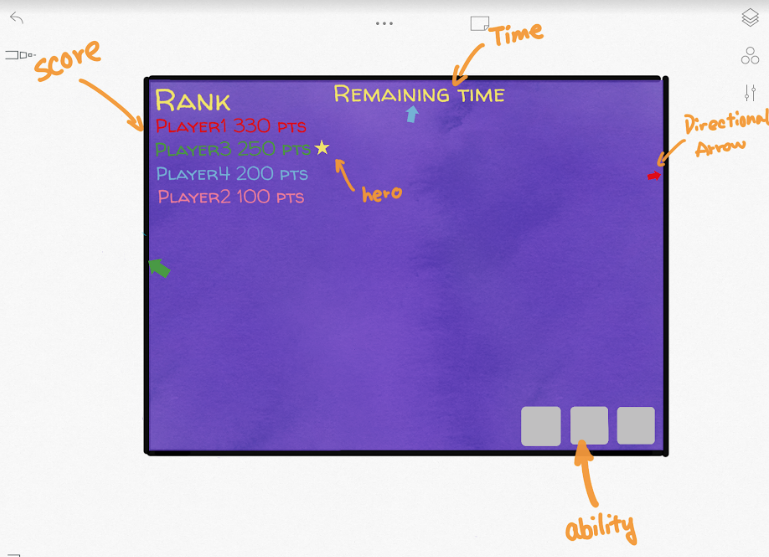
\includegraphics[width=0.8\linewidth]{images/ingame_ui.png}
  \caption{Early UI design. Directional arrows are less intrusive and easier to
  interpretive than a mini-map. Important information such as ability
cooldowns, score and time should be clearly visible to the player.}
\label{fig:ingame_ui}
\end{figure}

\begin{figure}[htpb]
  \centering
  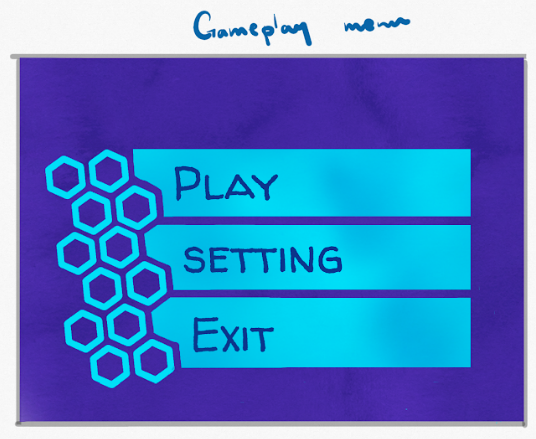
\includegraphics[width=0.8\linewidth]{images/main_menu.png}
  \caption{Possible design for the main menu with a Tron-like aestheic.}
\label{fig:main_menu}
\end{figure}

\begin{figure}[htpb]
  \centering
  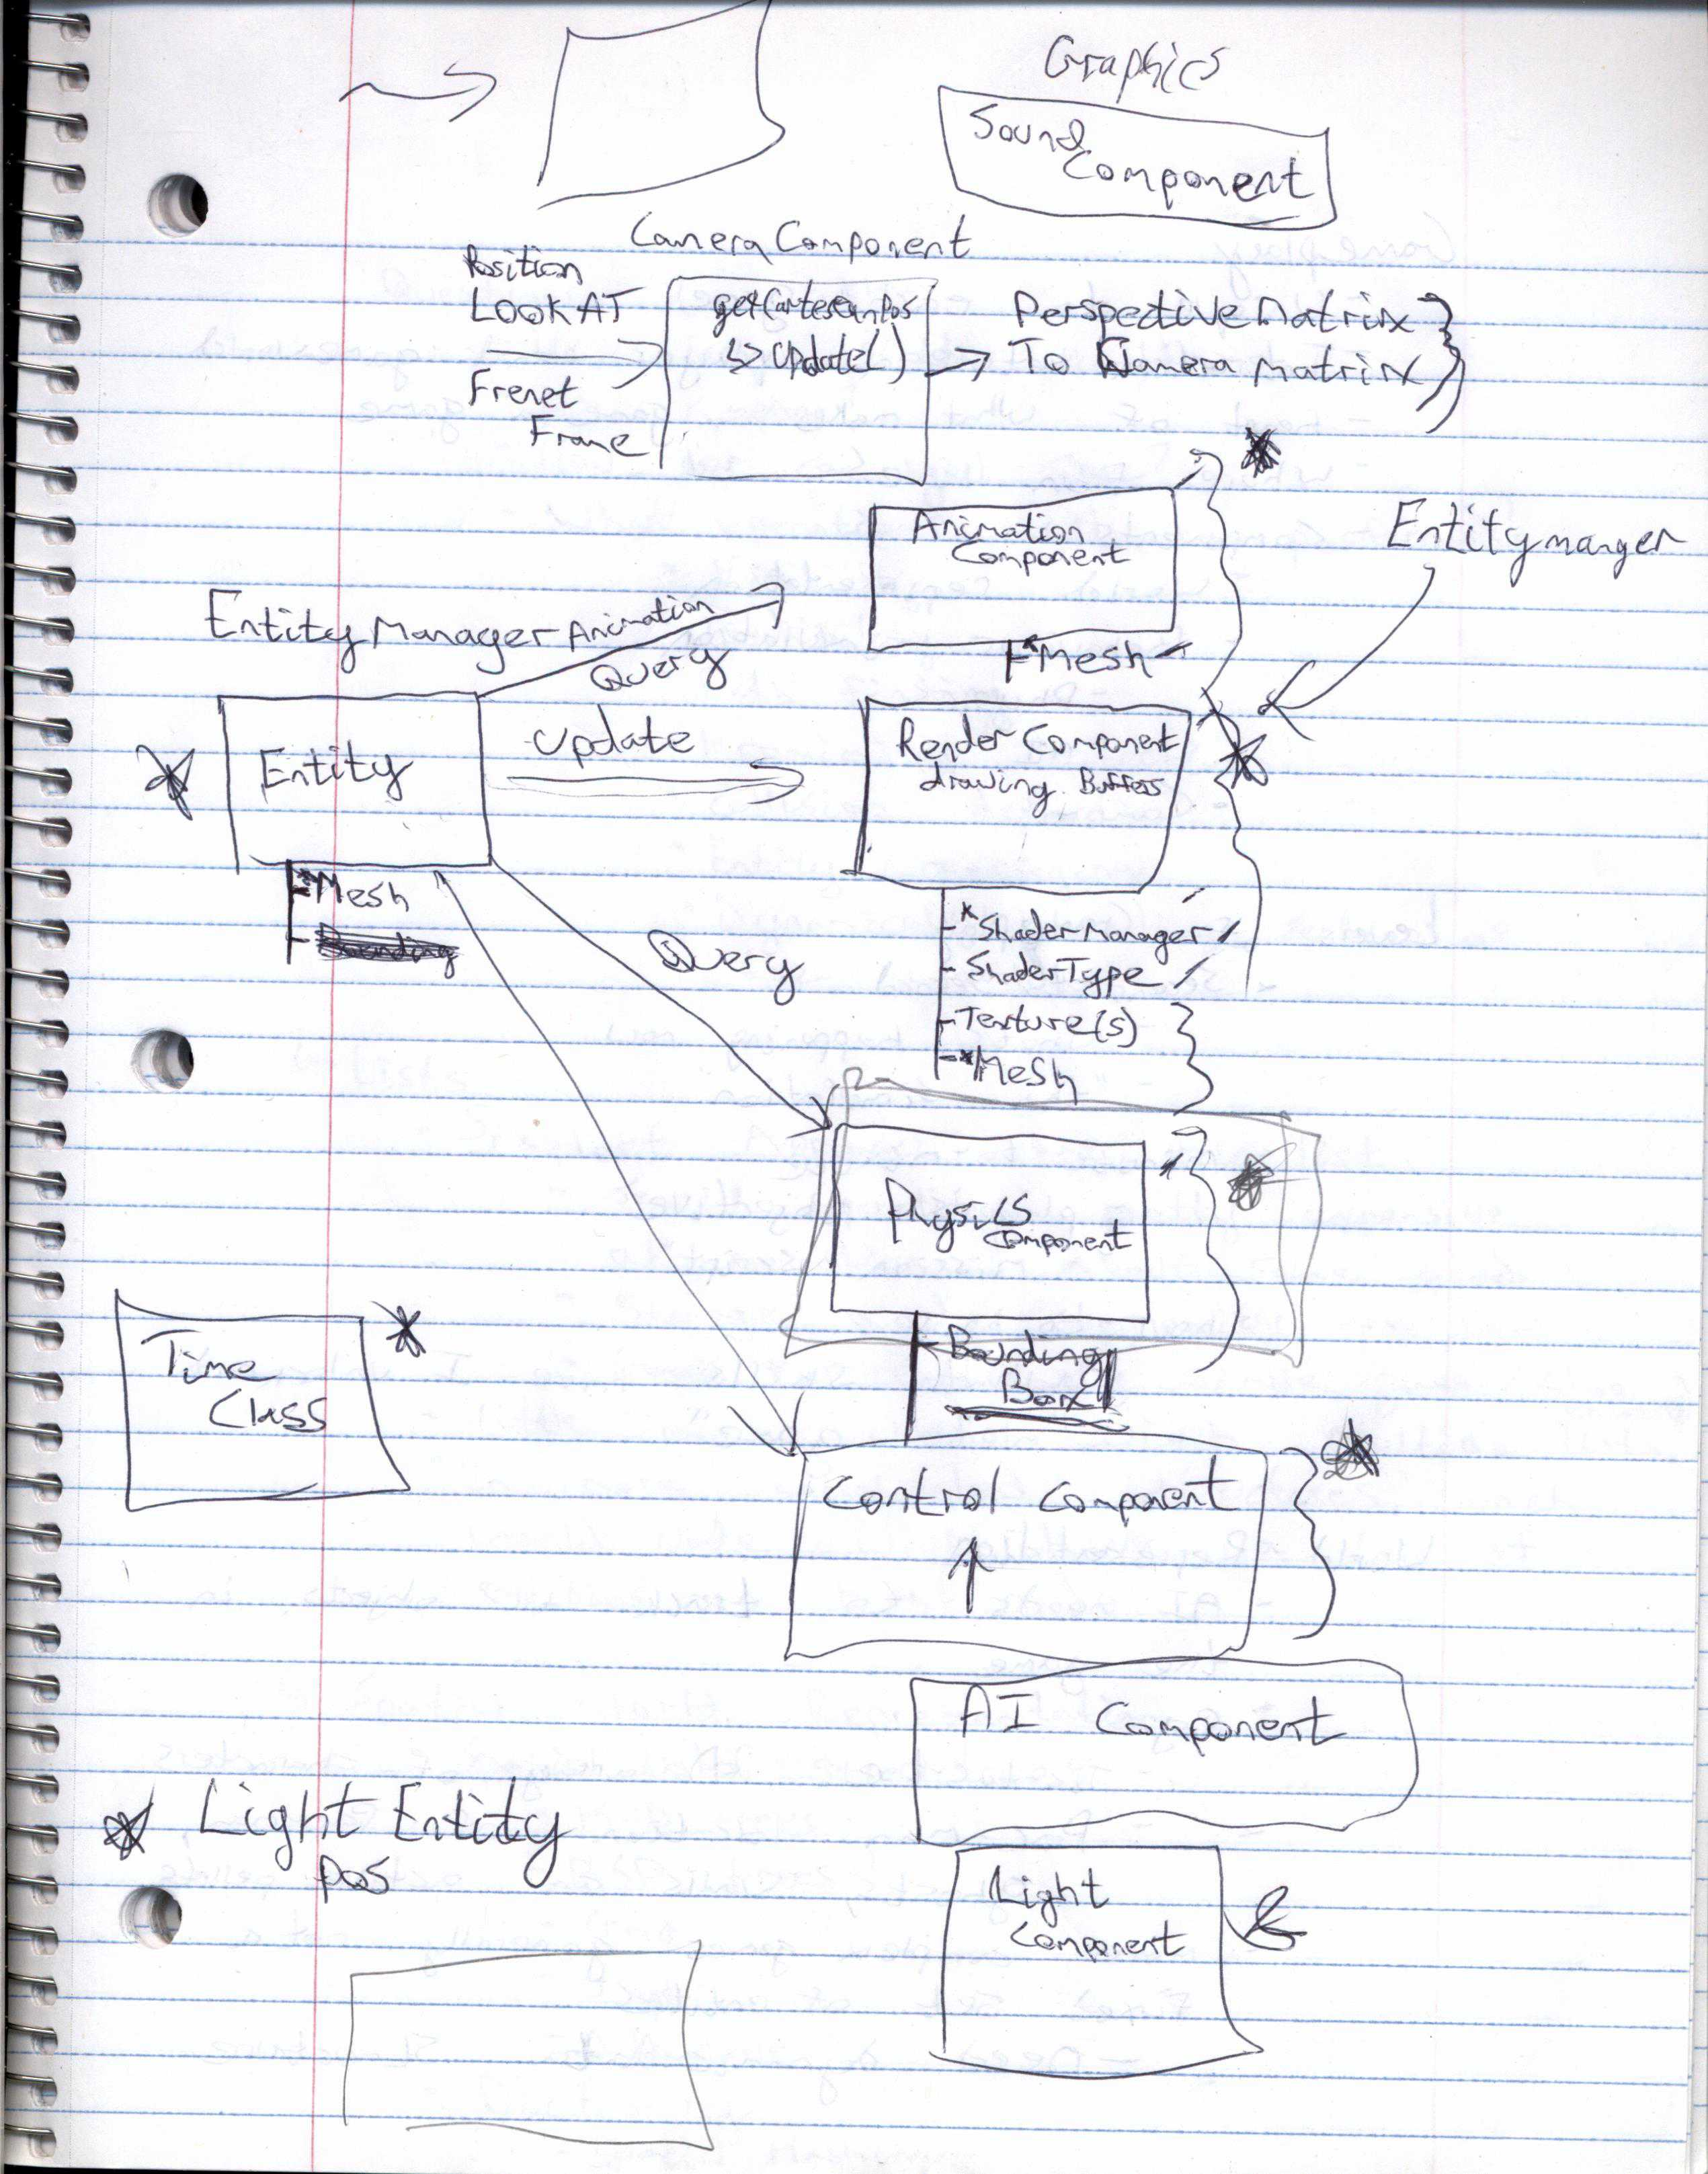
\includegraphics[width=0.8\linewidth]{images/Brainstorming_002.jpg}
  \caption{Early design of the game application framework}
\label{fig:Brainstorming_002}
\end{figure}

\end{document}
